\documentclass[12pt,a4paper]{report}

\usepackage[margin=1in]{geometry}
\usepackage{amsmath,amssymb}
\usepackage{booktabs,longtable,tabularx,array}
\usepackage{graphicx}
\usepackage{float}
\usepackage{enumitem}
\usepackage{tikz}
\usepackage{hyperref}
\usepackage{setspace}
\usepackage{microtype}
\hypersetup{colorlinks=true,linkcolor=black,citecolor=black,urlcolor=blue}
\setstretch{1.15}
\setlist{nosep,leftmargin=1.5em}
\setlength{\parskip}{0.35em}
\renewcommand{\arraystretch}{1.2}
\usetikzlibrary{arrows.meta,positioning,shapes.geometric}

\begin{document}

% -----------------------------------------------------------------------------
% Title page
% -----------------------------------------------------------------------------
\begin{titlepage}
\centering
{\Large PURBANCHAL UNIVERSITY\par}
\vspace{1.1cm}
{\large DEPARTMENT OF COMPUTER ENGINEERING\par}
{\large KHWOPA ENGINEERING COLLEGE\par}
{\normalsize LIBALI-08, BHAKTAPUR\par}
\vspace{1.5cm}
{\Large\bfseries A PROJECT FINAL-DEFENCE REPORT\par}
\vspace{0.4cm}
{\large ON\par}
\vspace{0.35cm}
{\LARGE\bfseries NutriAI: Personalized Meal Planner and Calorie Tracker\par}
\vspace{1cm}
\begin{minipage}{0.86\textwidth}
\centering
Project work submitted in partial fulfillment of the requirements for the degree of
Bachelor of Engineering in Computer Engineering (Seventh Semester).
\end{minipage}
\vfill
{\large Submitted by\par}
\vspace{0.3cm}
\begin{tabular}{lr}
Dristi Shrestha & (790313)\\
Prashant Ghimire & (790328)\\
Romina Koju & (790332)\\
Shrijan Sainju & (790342)
\end{tabular}
\vspace{1cm}

{\large UNDER THE SUPERVISION OF\par}
{\large Er. Avijit Karn\par}
\vfill
{\large 17 November 2026\par}
\end{titlepage}

\pagenumbering{roman}
\chapter*{Acknowledgement}
We express our sincere gratitude to Purbanchal University and Khwopa Engineering
College for providing the academic environment in which this project was developed.
We thank our supervisor, Er. Avijit Karn, for his guidance, feedback, and support
throughout the project. We also thank our families and friends for their encouragement,
and acknowledge the contributions of all team members in developing NutriAI and
preparing this report.

\vspace{1cm}
\noindent With regards,\\
Dristi Shrestha (790313)\\
Prashant Ghimire (790328)\\
Romina Koju (790332)\\
Shrijan Sainju (790342)

\chapter*{Abstract}
NutriAI is a web-based nutrition management system that combines a structured food
catalog, per-portion meal logging, deterministic personal nutrition calculations, rule-based
food eligibility, machine-learning food-quality scoring, and a tool-enabled conversational
assistant. The application is implemented with Django, PostgreSQL, Django REST
Framework, HTML templates, and JavaScript. The current live food catalog contains
1,475 records. The active CSV provenance field identifies 977 records from
\texttt{nutrition\_combined.csv (Indian Dishes)} and 498 from Nepal FCT 2012 (DFTQC).
Of these, 1,043 are marked recommendable, edible, and not supplements. A separate
catalog was assembled by extracting records from multiple sources and cleaning them to
meet the project's nutrition, classification, and recommendation requirements.

The recommendation training script uses seven nutrient features and a deterministic
nutrition-quality target. It trains an XGBoost regressor and a Random Forest regressor
on the same 80:20 random split. In a reproducible run on the current database, XGBoost
achieved lower holdout MAE and RMSE and higher $R^2$, accuracy, recall, and F1 than
Random Forest. These metrics measure agreement with the project's formula-generated
targets, not clinical outcomes or human preference. In the live ranking path, XGBoost is
the primary model; candidate eligibility, dietary restrictions, allergen exclusions, meal
filters, remaining-budget fit, and explicit likes/dislikes are applied separately.

Users can enter food portions in grams; the application scales per-100-g nutrient values
by portion size and updates daily totals. Personalized calorie targets are derived from
profile-based TDEE and the selected goal, with a manual target override. The Groq-based
assistant uses function tools to access the authenticated user's profile and allergies,
recent meal history, current food suggestions, and saved food preferences. The system
is a nutrition-support application, not a medical diagnostic or treatment service.

\noindent\textbf{Keywords:} Personalized Nutrition, Nepali Food, Meal Logging,
Calorie Tracking, XGBoost, Random Forest, PostgreSQL, Allergen Filtering,
Tool-Calling Conversational AI.

\tableofcontents
\listoftables
\listoffigures
\chapter*{List of Abbreviations}
\begin{longtable}{ll}
AI & Artificial Intelligence\\
API & Application Programming Interface\\
BMR & Basal Metabolic Rate\\
CSV & Comma-Separated Values\\
DRF & Django REST Framework\\
FCT & Food Composition Table\\
FDC & FoodData Central\\
LLM & Large Language Model\\
MAE & Mean Absolute Error\\
ML & Machine Learning\\
MSE & Mean Squared Error\\
ORM & Object-Relational Mapping\\
RF & Random Forest\\
RMSE & Root Mean Squared Error\\
TDEE & Total Daily Energy Expenditure\\
XGBoost & Extreme Gradient Boosting
\end{longtable}

\clearpage
\pagenumbering{arabic}

% -----------------------------------------------------------------------------
\chapter{Introduction}
% -----------------------------------------------------------------------------
\section{Background}
Nutritional requirements vary with age, sex, body size, activity level, goals, dietary
preferences, and allergies. A useful nutrition application must therefore do more than
show a generic meal list: it should keep a traceable food catalog, estimate individual
energy targets, record the portion actually eaten, and respect hard dietary restrictions.
NutriAI combines those functions in a web application with attention to Nepali foods and
local dietary practice.

The project separates deterministic calculation and safety rules from machine-learning
scores and language-model responses. Deterministic calculations supply repeatable
numbers; the recommender ranks eligible food records; and the conversational assistant
explains information using server-side tools. This separation is important because
language-model output is not treated as an authoritative source of calories or allergen
safety.

\section{Problem Definition}
Generic food applications may have limited representation of local dishes, rely on
standardized portions that do not match what a person ate, or display suggestions without
filtering food preparation ingredients from ready-to-eat choices. They may also fail to
adapt a daily calorie budget to a person's profile or provide an explanation of how a
suggestion relates to the remaining budget. NutriAI addresses these issues through a
labeled food catalog, gram-based logging, profile-derived calorie targets, candidate
eligibility checks, budget-aware ranking, and a conversational interface.

\section{Objectives}
\begin{enumerate}
  \item Maintain a structured catalog with nutrition, source, portion, and suitability
        attributes.
  \item Calculate a user's BMR, TDEE, goal-adjusted calorie target, and macro targets
        from profile characteristics.
  \item Record actual meal portions in grams and scale nutrients from per-100-g food
        values.
  \item Exclude catalog entries that are not marked recommendable and edible, as well
        as supplements, before ranking.
  \item Rank eligible foods using model-predicted nutrition quality, current budget fit,
        and saved feedback.
  \item Provide filterable meal suggestions and an authenticated conversational assistant
        with tool access to relevant user data.
\end{enumerate}

\section{Scope and Applications}
NutriAI supports personal nutrition tracking, food discovery, meal ideas, profile-based
targets, and general nutrition questions. It is not a clinical system, does not diagnose
conditions, and does not replace a registered dietitian or physician. The current system
has an operational recommendation endpoint; it should not be described as a clinically
validated diet prescription system.

\section{Contributions of the Final Prototype}
Since the mid-term prototype, the project has added or completed: a labeled 1,475-row
catalog import; hard eligibility flags for recommendation candidates; live XGBoost-based
ranking with budget and feedback terms; multiple simultaneous recommendation filters
and a single meal-time filter; gram-based meal logging; goal-adjusted calorie and macro
targets; allergen-aware food filtering; chatbot tools for profile/allergy, meal history,
recommendations, and likes/dislikes; and automated regression tests for these workflows.

% -----------------------------------------------------------------------------
\chapter{Related Work and Research Gap}
% -----------------------------------------------------------------------------
\section{Related Work}
Research on AI in nutrition has examined dietary assessment, personalized nutrition,
food recommendation, and conversational support. Reviews emphasize that personalized
systems depend on the quality and coverage of the underlying food data and on careful
handling of user-specific restrictions. Food recommender studies commonly combine
nutritional properties with user preferences and context. Ensemble tree methods such as
Random Forest and XGBoost are widely used on structured tabular features
\cite{breiman2001,chen2016}. Food-composition repositories and national food tables
provide standardized data that can support nutrition applications.

Conversational systems can make nutrition information easier to query, but generated
answers must be grounded in reliable application data and should not be presented as
clinical decisions. NutriAI therefore uses server-side function tools for profile, meal,
preference, and recommendation data, and retains deterministic code for calculations and
hard eligibility rules.

\section{Research Gap}
The project focuses on unifying culturally relevant food records, per-portion tracking,
personalized energy targets, eligibility filtering, recommendation ranking, and
conversation in a single student-scale application. The current work also exposes a
limitation that must be considered in evaluation: the ML target is a designed nutrition
quality formula rather than expert-rated or user-outcome labels. The system is consequently
a prototype recommender whose quality is measured first against its own defined target
and functional requirements, not a clinically validated personalized nutrition model.

% -----------------------------------------------------------------------------
\chapter{Project Management}
% -----------------------------------------------------------------------------
\section{Feasibility}
\textbf{Technical:} Python and Django provide the web and data layer; PostgreSQL stores
profiles, foods, logs, and preference history; XGBoost and scikit-learn support structured
model training; and the OpenAI-compatible client connects the chatbot to Groq.
\textbf{Economic:} the application uses open-source libraries, with external LLM API
usage as the principal potential operating cost. \textbf{Operational:} the user workflow
is conventional: register, complete a profile, select a meal or food portion, review
consumption, and ask the assistant a question.

\section{Technology Stack}
\begin{longtable}{p{0.25\textwidth}p{0.66\textwidth}}
\toprule
Layer & Current implementation\\
\midrule
Language & Python 3.12 environment\\
Web framework & Django 6.1.1\\
API framework & Django REST Framework 3.18.1\\
Database & PostgreSQL\\
Frontend & Django templates, HTML, CSS, JavaScript\\
ML & XGBoost 3.4.1 and scikit-learn 1.9.0 Random Forest\\
Chat assistant & Groq API using the OpenAI-compatible Python client\\
Model persistence & Joblib serialized estimators\\
\bottomrule
\end{longtable}

\section{Work Breakdown and Status}
\begin{longtable}{p{0.37\textwidth}p{0.18\textwidth}p{0.37\textwidth}}
\toprule
Work area & Status & Evidence in the current repository\\
\midrule
Requirements and application structure & Implemented & Django project and two application modules\\
Food-data integration & Implemented & Labeled CSV import command and persisted food fields\\
Profile and deterministic nutrition & Implemented & Profile models, calculation service, and dashboard integration\\
Meal, water, and weight tracking & Implemented & User-owned log models and views\\
Recommendation ranking & Implemented & Authenticated API, trained model loading, filter and score logic\\
Feedback handling & Implemented & Per-user recommendation feedback endpoint and history model\\
Conversational assistant & Implemented & Groq API service and user-scoped function tools\\
Testing & Implemented at prototype level & Explicit Django tests for imports, logging, targets, tools, and ranking\\
Deployment and clinical validation & Not established & Requires production hosting, data governance, and expert evaluation\\
\bottomrule
\end{longtable}

% -----------------------------------------------------------------------------
\chapter{Data and Knowledge-Base Construction}
% -----------------------------------------------------------------------------
\section{Active Runtime Dataset}
The live importer reads \texttt{myapp/data/destination\_with\_food\_attributes.csv}.
The inspected file has 1,475 rows, 1,475 distinct \texttt{food\_id} values, and no
missing entries in the seven inspected nutrition columns (calories, protein,
carbohydrates, fat, fiber, sugar, sodium). The active PostgreSQL database also contains
1,475 Food rows at the time of this report.

\begin{table}[H]
\centering
\caption{Current runtime catalog summary}
\begin{tabular}{lr}
\toprule
Measure & Count\\
\midrule
CSV food records & 1,475\\
Distinct food IDs & 1,475\\
Database food records & 1,475\\
Eligible: recommendable, edible, not supplement & 1,043\\
Not marked recommendable & 432\\
Marked edible & 1,468\\
Marked non-edible & 7\\
Marked as supplement & 1\\
\bottomrule
\end{tabular}
\end{table}

\section{Source Provenance and Dataset Caution}
The fixed catalog was assembled by extracting food records from multiple sources and
cleaning the records to meet the application's nutrition and classification requirements.
The current CSV's \texttt{data\_source} field records 977 rows as
\texttt{nutrition\_combined.csv (Indian Dishes)} and 498 as Nepal FCT 2012 (DFTQC).
These labels provide traceability for the sources represented in the active catalog.

\section{Food Attributes and Eligibility}
The labeled CSV includes nutrition, serving size, dietary flags, provenance, food type,
meal category, preparation state, recommendation group, and three explicit eligibility
fields: \texttt{is\_recommendable}, \texttt{is\_edible\_food}, and
\texttt{is\_supplement}. Its food-type distribution is summarized below.

\begin{table}[H]
\centering
\caption{Food-type distribution in the active CSV}
\begin{tabular}{lr}
\toprule
Food type & Rows\\
\midrule
food & 805\\
snack & 237\\
meal & 54\\
ingredient & 372\\
herbal product & 6\\
supplement & 1\\
\midrule
Total & 1,475\\
\bottomrule
\end{tabular}
\end{table}

The importer validates required headers, non-empty food names, finite numeric values,
and boolean fields before opening a database transaction. It uses the CSV food ID as a
stable source key, preserves duplicate names with distinct IDs, and marks catalog records
absent from the active CSV as ineligible rather than deleting records referenced by past
logs. Recommendation candidates must be explicitly recommendable and edible and must
not be supplements.

\section{Dataset Cleaning and Normalization}
The extracted records were consolidated into a fixed CSV with a consistent schema.
Nutrition fields are numeric and expressed on the catalog's standard serving basis;
serving size, food category, dietary flags, allergen attributes, and source labels are
retained alongside each food. Classification fields identify the food type, suggested
meal categories, preparation state, and recommendation group. The dataset also includes
explicit labels for whether an item is recommendable, edible as presented, and a
supplement.

Before import, the data was reviewed for missing values, inconsistent representations,
duplicate identifiers, and records unsuitable for standalone recommendations. The
current CSV contains 1,475 unique food IDs and populated values in the seven nutrition
columns used by training. Foods may still be useful as ingredients or components while
being excluded as standalone suggestions; the recommendation eligibility label captures
that distinction. The import command validates the required columns and value formats
before updating the PostgreSQL catalog.

\section{Data Limitations}
The current audit establishes row counts and populated fields, not that every value has
been independently verified against its original source. Some CSV records derive from a
compiled dataset and some from Nepal FCT. Nutrition values can vary by recipe, cooking
method, water content, and serving definition. Allergen coverage is only as reliable as
the source tags and profile data. Future dataset releases should retain source URL or
citation, retrieval date, original serving definition, conversion method, and review
status per record.

% -----------------------------------------------------------------------------
\chapter{System Methodology and Architecture}
% -----------------------------------------------------------------------------
\section{Architecture}
NutriAI has two Django applications. \texttt{myapp} implements accounts, profile forms,
food logging, core pages, and chatbot orchestration. \texttt{recommendations} implements
the meal-planner page, recommendation API, feedback endpoint, and quick-log endpoint.
Django ORM models persist the user, catalog, meal logs, profile restrictions, and
recommendation feedback in PostgreSQL.

\begin{center}
\fbox{\parbox{0.91\textwidth}{
Browser (Django templates and JavaScript)\\[0.2em]
$\downarrow$ authenticated HTTP request\\[0.2em]
Django views and DRF endpoints\\[0.2em]
$\rightarrow$ PostgreSQL models for profile, foods, logs, and feedback\\[0.2em]
$\rightarrow$ deterministic nutrition calculations and rule-based filters\\[0.2em]
$\rightarrow$ XGBoost / hybrid ranking for current food suggestions\\[0.2em]
$\rightarrow$ Groq conversational model with server-side function tools
}}
\end{center}

The browser-facing application uses Django session authentication and CSRF protection.
DRF endpoints require authenticated users. Food, profile, meal-history, and preference
queries are scoped to the current authenticated user where applicable. The chatbot does
not receive a user's database identity as model-provided input; tool implementations
receive the authenticated user from the server.

\section{Data-Flow Diagram}
Figure~\ref{fig:data-flow} shows how the fixed catalog, user profile, meal logs, and
recommendation feedback contribute to food suggestions and daily tracking. The CSV
enters PostgreSQL through the validating import command. At request time, the
recommendation endpoint applies eligibility and user-specific filters before scoring the
remaining foods. A quick-log action writes scaled nutrients to the meal log, which feeds
the next daily-budget calculation.

\begin{figure}[H]
\centering
\resizebox{\textwidth}{!}{%
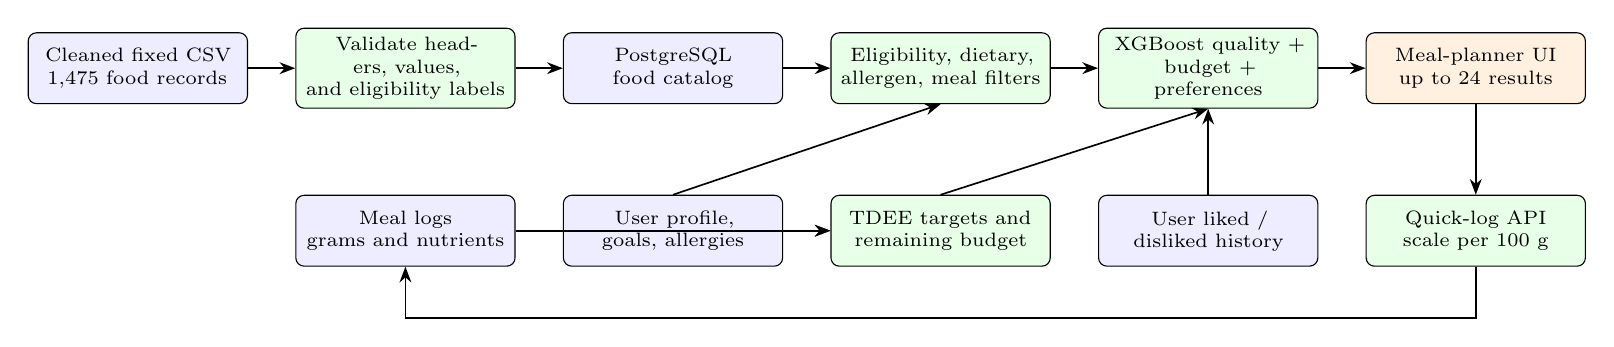
\begin{tikzpicture}[
      data/.style={draw,rounded corners=3pt,fill=blue!7,align=center,text width=2.55cm,minimum height=0.9cm,font=\scriptsize},
      process/.style={draw,rounded corners=3pt,fill=green!9,align=center,text width=2.55cm,minimum height=0.9cm,font=\scriptsize},
      user/.style={draw,rounded corners=3pt,fill=orange!12,align=center,text width=2.55cm,minimum height=0.9cm,font=\scriptsize},
      flow/.style={-{Stealth[length=2mm]},semithick},
      node distance=0.75cm and 0.6cm
]
\node[data] (csv) {Cleaned fixed CSV\\1,475 food records};
\node[process,right=of csv] (import) {Validate headers, values,\\and eligibility labels};
\node[data,right=of import] (catalog) {PostgreSQL\\food catalog};
\node[process,right=of catalog] (filter) {Eligibility, dietary,\\allergen, meal filters};
\node[process,right=of filter] (rank) {XGBoost quality +\\budget + preferences};
\node[user,right=of rank] (page) {Meal-planner UI\\up to 24 results};

\node[data,below=1.15cm of catalog] (profile) {User profile,\\goals, allergies};
\node[data,left=of profile] (logs) {Meal logs\\grams and nutrients};
\node[process,right=of profile] (budget) {TDEE targets and\\remaining budget};
\node[data,right=of budget] (feedback) {User liked /\\disliked history};
\node[process,right=of feedback] (quicklog) {Quick-log API\\scale per 100 g};

\draw[flow] (csv) -- (import);
\draw[flow] (import) -- (catalog);
\draw[flow] (catalog) -- (filter);
\draw[flow] (filter) -- (rank);
\draw[flow] (rank) -- (page);
\draw[flow] (profile.north) -- (filter.south);
\draw[flow] (profile) -- (budget);
\draw[flow] (logs) -- (budget);
\draw[flow] (budget.north) -- (rank.south);
\draw[flow] (feedback.north) -- (rank.south);
\draw[flow] (page.south) -- (quicklog.north);
\draw[flow] (quicklog.south) -- ++(0,-0.65) -| (logs.south);
\end{tikzpicture}%
}
\caption{NutriAI data flow for catalog import, personalized ranking, and meal tracking.}
\label{fig:data-flow}
\end{figure}

\section{User Profile and Energy Calculation}
The profile stores date of birth, gender, height, weight, activity level, goal, optional
manual daily calorie target, allergies, and dietary tags. Age is derived from date of
birth. BMR is calculated with the Mifflin--St Jeor equations for male and female
profiles. For other/unspecified gender values, the code uses an approximate constant of
$-78$ in the same equation; this is a project-specific approximation, not a clinically
validated equation for every population.

\begin{align}
BMR_{male} &= 10W + 6.25H - 5A + 5,\\
BMR_{female} &= 10W + 6.25H - 5A - 161,\\
BMR_{other} &= 10W + 6.25H - 5A - 78,\\
TDEE &= BMR \times a.
\end{align}
Here $W$ is weight in kilograms, $H$ is height in centimetres, $A$ is age in years, and
$a$ is the activity multiplier. The implemented multipliers are 1.20 (sedentary), 1.375
(light), 1.55 (moderate), and 1.725 (very active).

An optional manually entered calorie target overrides the computed value. Otherwise,
the current code sets the goal target to 85\% of TDEE for weight loss, 100\% for
maintenance, and 110\% for weight gain. Protein is estimated at 1.2 g per kg body
weight when weight is present; fat is set to 30\% of target calories; carbohydrates use
the remaining energy after protein and fat. If the required profile data is incomplete,
the code falls back to a general calorie target. The current code does not calculate BMI;
BMI was discussed in the mid-term report but should not be claimed as an operational
feature in this final report.

\section{Gram-Based Meal Tracking}
Catalog nutrition fields are stored per 100 g. If a user logs $q$ grams, each nutrient $x$
is calculated as
\begin{equation}
x_{consumed} = x_{per\,100g} \times \frac{q}{100}.
\end{equation}
Both dashboard logging and the meal-planner quick-log save the portion in grams and
store scaled calories, protein, carbohydrates, fat, and fiber. The dashboard displays
logged calories for each recent meal. The quick-log API returns an updated daily budget
so the meal planner can refresh its calorie and macro summary immediately.

\section{Dietary, Allergen, and Suitability Filtering}
Hard eligibility gates are applied before ranking:
\begin{itemize}
      \item \texttt{is\_recommendable} must be true;
      \item \texttt{is\_edible\_food} must be true;
      \item \texttt{is\_supplement} must be false.
\end{itemize}
User dietary settings, supported health-condition checks, allergy tags, and custom
allergy text are also used to filter candidates. Meal-time categories and page-selected
filters are applied before scoring and before the top-24 limit. This prevents raw
ingredient rows from occupying recommendation slots when the CSV identifies them as
non-recommendable.

\section{Live Recommendation Ranking}
For each eligible food, the API constructs a seven-feature vector:
calories, protein, carbohydrates, fat, fiber, sugar, and sodium. The saved XGBoost
regressor predicts a nutrition-quality score. The final score combines that output with
budget fit and saved user feedback:
\begin{equation}
S = 0.50S_{XGB} + 0.30S_{budget} + 0.20S_{preference}.
\end{equation}
Budget fit uses cosine similarity between remaining macro/calorie budget and a food
feature vector. The preference signal is 1.0 for liked foods, 0.0 for disliked foods, and
0.5 where no feedback exists. These fixed weights are implementation constants, not
weights learned from user outcome data. The API sorts by score and returns up to 24
foods. The meal-planner interface supports simultaneous preference filters and one
meal-time choice, then requests a newly filtered and ranked result set on Refresh.

\section{Conversational Assistant and Tool Calling}
The conversational assistant is implemented as a server-mediated tool-calling workflow.
The browser sends the user's text to an authenticated Django view, which attaches a
bounded conversation history and submits the request to the Groq-hosted language model
through an OpenAI-compatible client. The model may answer directly or request one or
more backend functions. Django executes each requested function using the authenticated
request user, appends the structured result to the conversation, and asks the model to
produce the final natural-language answer.

\begin{center}
\fbox{\parbox{0.9\textwidth}{
User question\quad $\rightarrow$\quad Django chatbot view\quad $\rightarrow$\quad
Groq model selects tool(s)\par\medskip
$\leftarrow$ final answer\quad $\leftarrow$ model uses tool results\quad
$\leftarrow$ Django runs user-scoped database/recommender functions
}}
\end{center}

The available functions are summarized in Table~\ref{tab:chatbot-tools}. Tool outputs
are JSON objects with only the fields needed to answer the question. Limits on date
windows and result counts avoid returning an unbounded history or recommendation list.

\begin{table}[H]
\centering
\caption{User-scoped chatbot tools}
\label{tab:chatbot-tools}
\small
\begin{tabularx}{\textwidth}{p{0.29\textwidth}p{0.62\textwidth}}
\toprule
Tool & Information returned and use\\
\midrule
Profile and allergy lookup & Profile characteristics, goal, calorie target,
selected allergens, and custom allergy text. Used for profile-aware nutrition responses.\\
Recent meal history & Recent meal names, times, meal types, logged
gram portions, calories, and macros. Defaults to seven days and ten records, with
bounded caller-selected limits.\\
Current personalized suggestions & Current suggestions from the
same recommendation engine used by the meal planner. Returns a small bounded set.\\
Saved food preferences & Foods this user marked liked or disliked,
including food category and recommendation group.\\
\bottomrule
\end{tabularx}
\end{table}

\subsection{Tool Selection and Multi-Step Questions}
The model is instructed to use the profile tool before giving personalized food advice,
the meal-history tool when asked what the user has eaten, the preference tool when asked
what foods the user likes or avoids, and the recommender tool when asked for ideas. A
question such as ``What have I eaten recently, and what should I try next?'' can require
both meal-history and recommendation calls. The service supports sequential tool-call
rounds before returning a final answer. The chatbot is not a retrieval-augmented
generation system: there is no vector database or external reference-document search
implementation in the current code.

\subsection{Sequence Diagram for a Personalized Chat Request}
Figure~\ref{fig:chat-sequence} traces a question that needs both meal-history and
recommendation context. The first model response requests profile and meal-history data;
the Django service fetches only the current user's records and returns structured tool
results. The model may then request current recommendations, which are generated by the
same filtered recommender used by the meal planner. After receiving those results, the
model produces a final answer and Django returns it to the browser. The diagram shows
the normal successful path; provider or configuration errors instead produce an
application error response.

\begin{figure}[H]
\centering
\resizebox{\textwidth}{!}{%
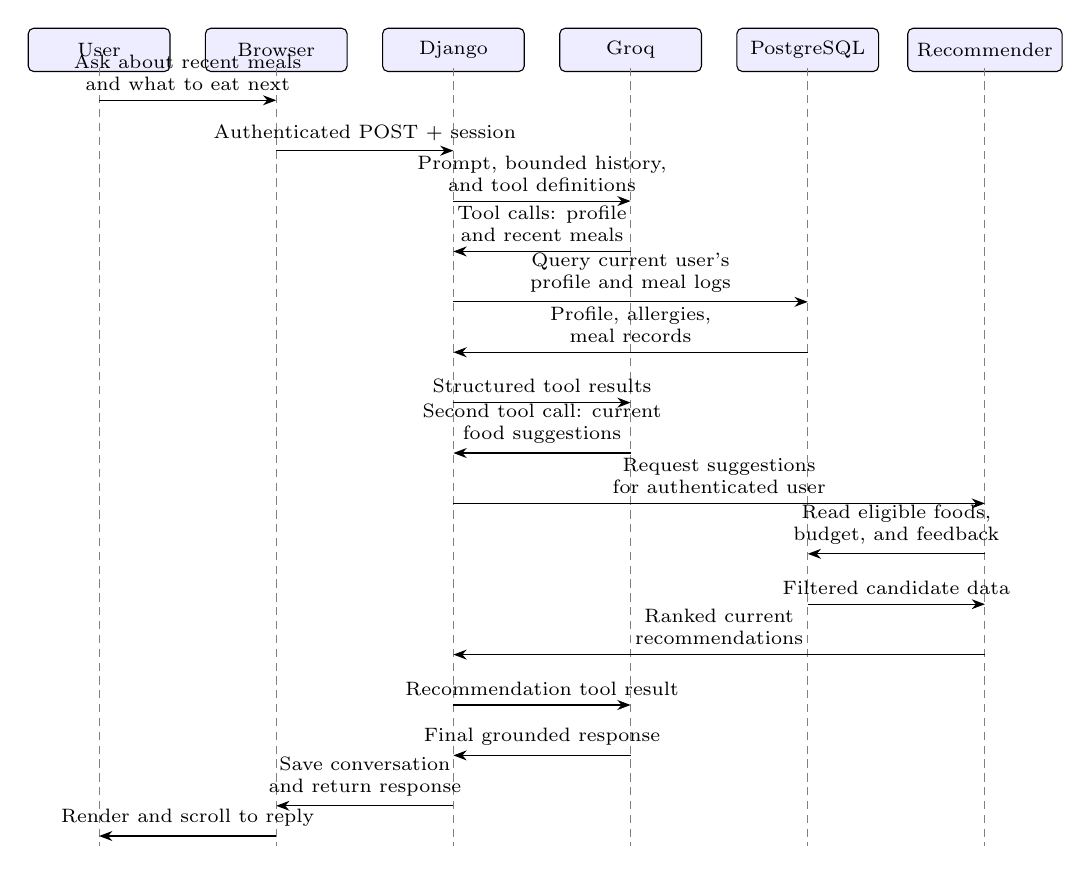
\begin{tikzpicture}[x=2.25cm,y=0.64cm,>=Stealth]
\foreach \x/\name in {0/User,1/Browser,2/Django,3/Groq,4/PostgreSQL,5/Recommender} {
      \node[draw,rounded corners=2pt,fill=blue!7,minimum width=1.8cm,minimum height=0.55cm,align=center,font=\scriptsize] at (\x,0) {\name};
      \draw[densely dashed,gray] (\x,-0.35) -- (\x,-15.8);
}
\draw[->] (0,-1) -- node[above,font=\scriptsize,align=center]{Ask about recent meals\\and what to eat next} (1,-1);
\draw[->] (1,-2) -- node[above,font=\scriptsize]{Authenticated POST + session} (2,-2);
\draw[->] (2,-3) -- node[above,font=\scriptsize,align=center]{Prompt, bounded history,\\and tool definitions} (3,-3);
\draw[<-] (2,-4) -- node[above,font=\scriptsize,align=center]{Tool calls: profile\\and recent meals} (3,-4);
\draw[->] (2,-5) -- node[above,font=\scriptsize,align=center]{Query current user's\\profile and meal logs} (4,-5);
\draw[<-] (2,-6) -- node[above,font=\scriptsize,align=center]{Profile, allergies,\\meal records} (4,-6);
\draw[->] (2,-7) -- node[above,font=\scriptsize]{Structured tool results} (3,-7);
\draw[<-] (2,-8) -- node[above,font=\scriptsize,align=center]{Second tool call: current\\food suggestions} (3,-8);
\draw[->] (2,-9) -- node[above,font=\scriptsize,align=center]{Request suggestions\\for authenticated user} (5,-9);
\draw[->] (5,-10) -- node[above,font=\scriptsize,align=center]{Read eligible foods,\\budget, and feedback} (4,-10);
\draw[<-] (5,-11) -- node[above,font=\scriptsize]{Filtered candidate data} (4,-11);
\draw[<-] (2,-12) -- node[above,font=\scriptsize,align=center]{Ranked current\\recommendations} (5,-12);
\draw[->] (2,-13) -- node[above,font=\scriptsize]{Recommendation tool result} (3,-13);
\draw[<-] (2,-14) -- node[above,font=\scriptsize]{Final grounded response} (3,-14);
\draw[->] (2,-15) -- node[above,font=\scriptsize,align=center]{Save conversation\\and return response} (1,-15);
\draw[->] (1,-15.6) -- node[above,font=\scriptsize]{Render and scroll to reply} (0,-15.6);
\end{tikzpicture}%
}
\caption{Sequence of a multi-tool chatbot request for meal history and food suggestions.}
\label{fig:chat-sequence}
\end{figure}

\subsection{Privacy and Safety Boundaries}
The user identity used for each tool comes from the authenticated Django request, not
from an argument supplied by the language model. Meal history and saved feedback are
queried for that user only. Tool arguments are limited and capped in server-side code.
The system prompt asks the assistant not to diagnose medical conditions and to direct
medical concerns to qualified professionals. Allergen exclusion is enforced by the
recommendation engine as deterministic filtering; the language model is not the safety
boundary. Profile completeness, food tags, and source-data accuracy still limit the
strength of any personalization or allergy assurance.

The application stores recent conversation turns in the Django session, bounded to the
latest twelve entries. The service reports a configuration error if the Groq API key is
missing and a provider error if a call cannot be completed. The interface displays a
processing indicator, scrolls to the latest message, and renders a limited Markdown
subset (bold, italic, and inline code) only after escaping untrusted response text.

\subsection{Recommendation History Boundaries}
The recommendation tool returns current personalized suggestions using today's budget,
profile restrictions, and saved feedback. The database does not maintain an impression
snapshot of every recommendation card shown to the user. \texttt{RecommendationHistory}
stores feedback and related events, not every displayed list. Therefore the assistant can
discuss current suggestions and saved likes/dislikes, but must not claim to know the
exact contents of a past recommendation page unless impression logging is added.

% -----------------------------------------------------------------------------
\chapter{Machine-Learning Training and Evaluation}
% -----------------------------------------------------------------------------
\section{Model Purpose and Target Construction}
The ML model is a regression model that estimates a nutrition-quality score in the range
$[0,1]$. It is not a model that directly learns an individual's meal preferences. The
trainer loads foods satisfying the three catalog eligibility flags and creates seven
numeric nutrient features. A target score is generated with the following rule:
\begin{align}
p &= \operatorname{clip}(4P/C,0,1), & f &= \operatorname{clip}(F/10,0,1),\\
t &= 1-\operatorname{clip}(9T/C,0,1), & s &= 1-\operatorname{clip}(S/25,0,1),\\
n &= 1-\operatorname{clip}(Na/500,0,1),\\
y &= 0.35p + 0.20f + 0.20t + 0.15s + 0.10n.
\end{align}
Here $C$ is calories, $P$ protein in grams, $F$ fiber, $T$ fat, $S$ sugar, and $Na$
sodium in milligrams. The implementation uses floors to avoid division by zero and clips
the final target to $[0,1]$. Seventeen synthetic boundary samples are appended with
manually specified target values to represent very low through very high quality profiles.
Thus, the training target is a transparent project heuristic; it is not an expert-labeled
clinical ground truth or learned user rating.

\section{Training/Test Split and Reasoning}
The code calls \texttt{train\_test\_split} with \texttt{test\_size=0.20} and
\texttt{random\_state=42}. The 80\%
training portion is used to fit each regressor; the held-out 20\% is used to estimate
performance on samples not used by that fit. With the current database, 1,043 eligible
real foods plus 17 synthetic samples produce 1,060 rows: 848 training samples and 212
test samples. The fixed random seed makes this particular split reproducible. An 80:20
split is a practical baseline for a small dataset, but it is not cross-validation and does
not establish performance on independent future data.

\section{Algorithms and Hyperparameters}
\begin{longtable}{p{0.23\textwidth}p{0.68\textwidth}}
\toprule
Model & Configuration used by the trainer\\
\midrule
XGBoost regressor & 200 estimators; maximum depth 5; learning rate 0.08; row
subsample 0.8; column subsample 0.8; $L_1$ regularization (reg\_alpha) 0.1;
random seed 42. The default regression objective is squared error.\\
Random Forest regressor & 200 trees; maximum depth 8; minimum leaf size 2;
random seed 42; one parallel worker. The default regression split criterion is squared
error.\\
\bottomrule
\end{longtable}

Both models are trained and evaluated with the same split and continuous targets. MAE,
RMSE, and $R^2$ assess regression performance. For additional threshold-based
summaries, continuous target and prediction values are converted to binary classes at
0.5, then accuracy, precision, recall, and F1 are calculated. The threshold metrics are
secondary summaries; the core task remains regression.

\section{Measured Holdout Results}
The following metrics were reproduced in memory using the current database and the
same training split and hyperparameters. Model files were not overwritten during this
measurement.

\begin{table}[H]
\centering
\caption{Model performance on one 212-row held-out split}
\begin{tabular}{lrr}
\toprule
Metric & XGBoost & Random Forest\\
\midrule
MAE & 0.0106 & 0.0183\\
RMSE & 0.0172 & 0.0282\\
$R^2$ & 0.9694 & 0.9170\\
Accuracy at 0.5 & 0.9764 & 0.9481\\
Precision at 0.5 & 1.0000 & 1.0000\\
Recall at 0.5 & 0.7727 & 0.5000\\
F1 at 0.5 & 0.8718 & 0.6667\\
\bottomrule
\end{tabular}
\end{table}

On this split, XGBoost has lower MAE and RMSE and higher $R^2$, accuracy, recall, and
F1; precision is equal. The current application therefore loads XGBoost as its primary
quality-score model. Random Forest is trained and returned as a comparison score, but
its score is not included in the live hybrid ranking formula.

\section{Training Metric Visualizations}
The training program saves visual summaries alongside the serialized estimators in its
\texttt{training\_plots} output folder. Figure~\ref{fig:regression-metrics}
compares regression errors and fit scores, while Figure~\ref{fig:classification-metrics}
shows threshold-based classification metrics. The metrics are kept in separate figures
because their scales and interpretations differ.

\begin{figure}[H]
\centering
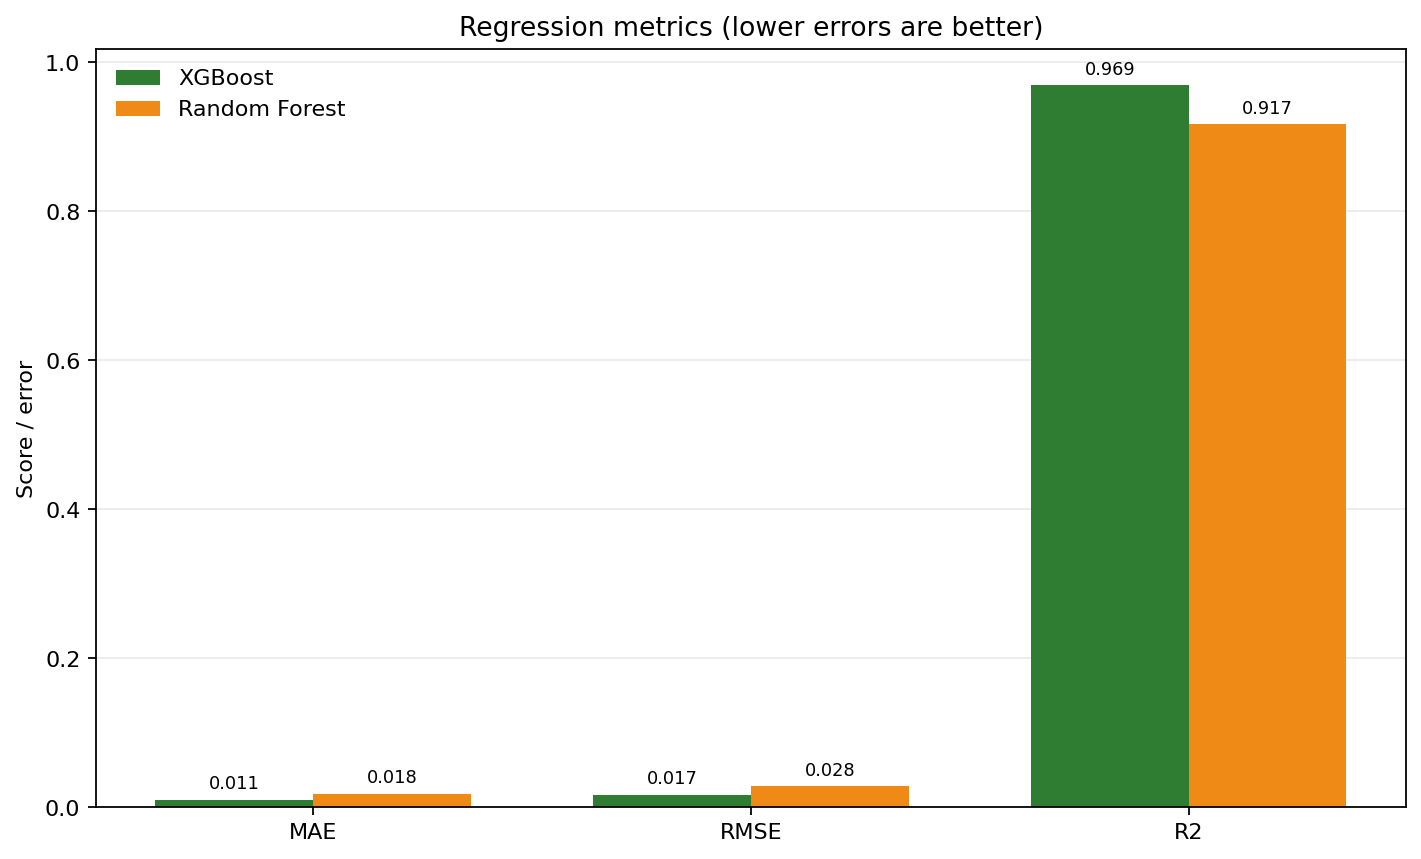
\includegraphics[width=0.82\textwidth,height=0.34\textheight,keepaspectratio]{recommendations/ml/training_plots/regression_metrics.png}
\caption{XGBoost and Random Forest regression metrics on the held-out split. Lower MAE and RMSE are better; higher $R^2$ is better.}
\label{fig:regression-metrics}
\end{figure}

\begin{figure}[H]
\centering
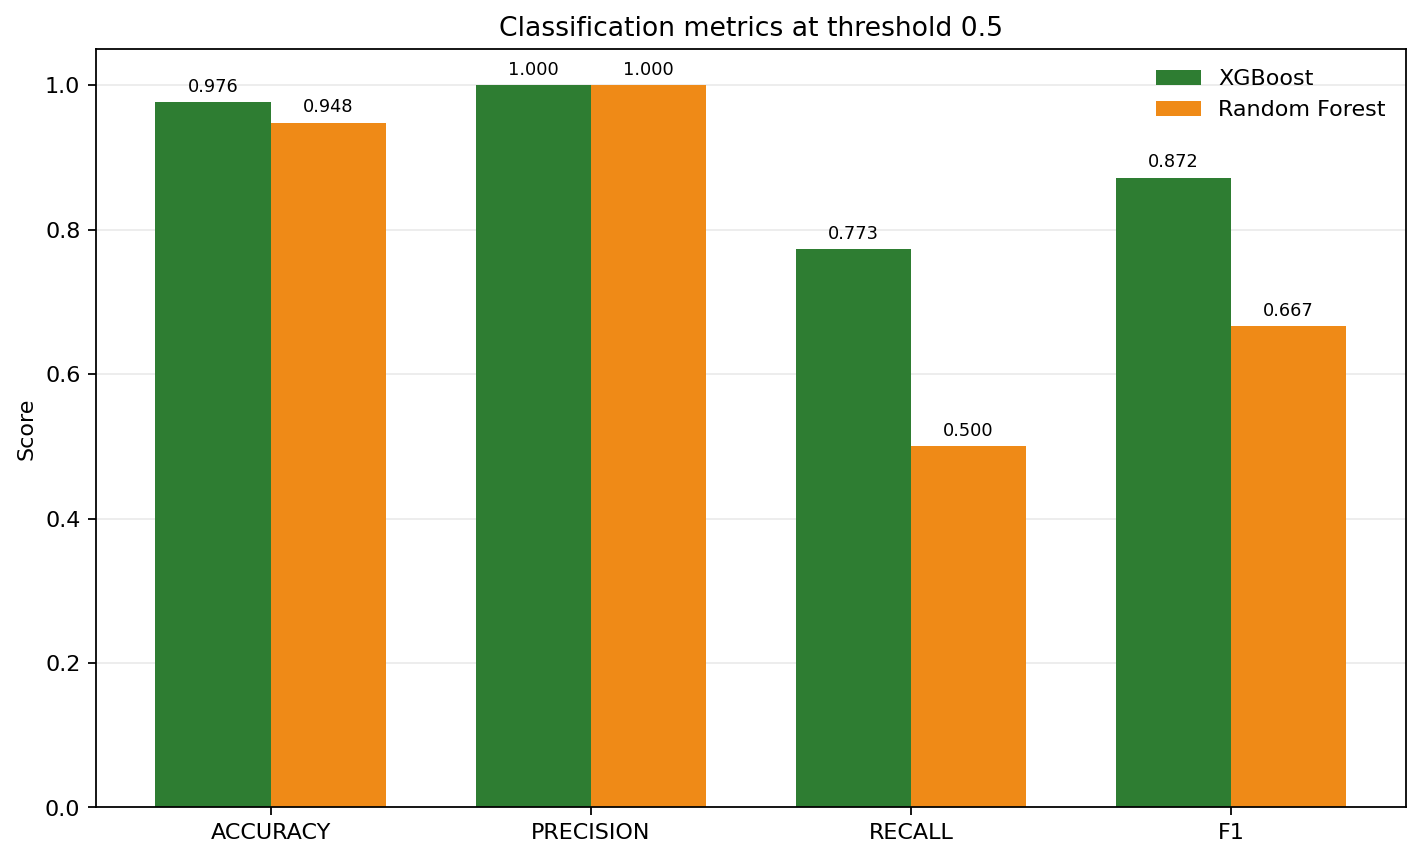
\includegraphics[width=0.82\textwidth,height=0.34\textheight,keepaspectratio]{recommendations/ml/training_plots/classification_metrics.png}
\caption{Accuracy, precision, recall, and F1 after thresholding the regression outputs at 0.5.}
\label{fig:classification-metrics}
\end{figure}

\clearpage
Figure~\ref{fig:actual-predicted} compares each model's predicted score with the
formula-generated target for individual held-out samples. Points nearer the dashed
identity line have smaller prediction errors. Figure~\ref{fig:feature-importance}
shows the models' built-in relative feature-importance values. Feature importance
describes the fitted models and must not be interpreted as causal evidence about health.

\begin{figure}[H]
\centering
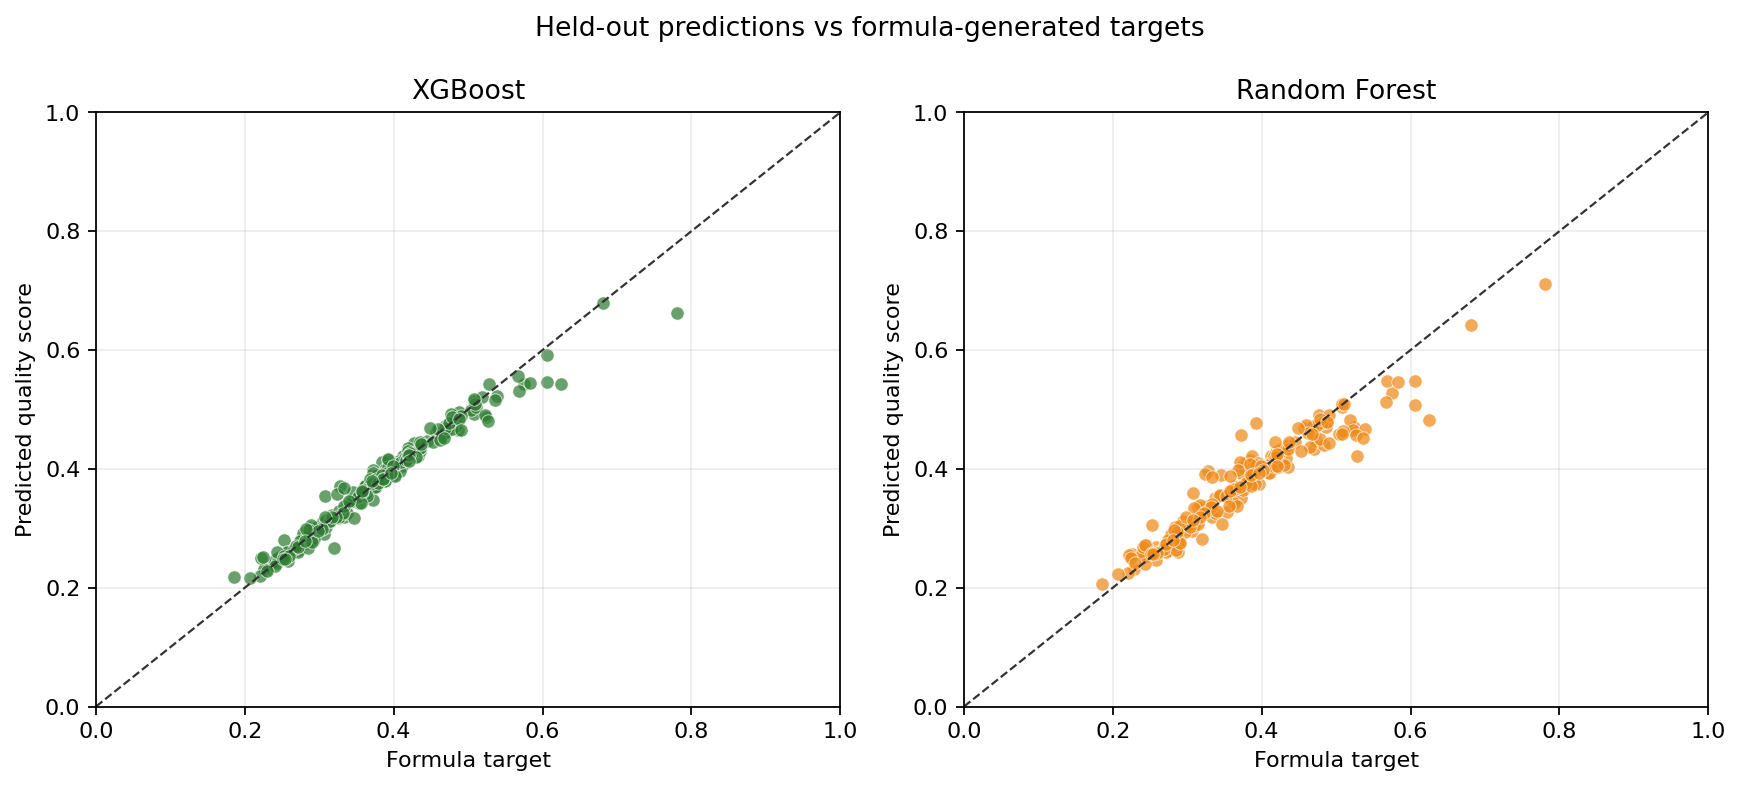
\includegraphics[width=0.82\textwidth,height=0.34\textheight,keepaspectratio]{recommendations/ml/training_plots/actual_vs_predicted.png}
\caption{Held-out actual target scores versus model predictions. The dashed line indicates perfect agreement.}
\label{fig:actual-predicted}
\end{figure}

\begin{figure}[H]
\centering
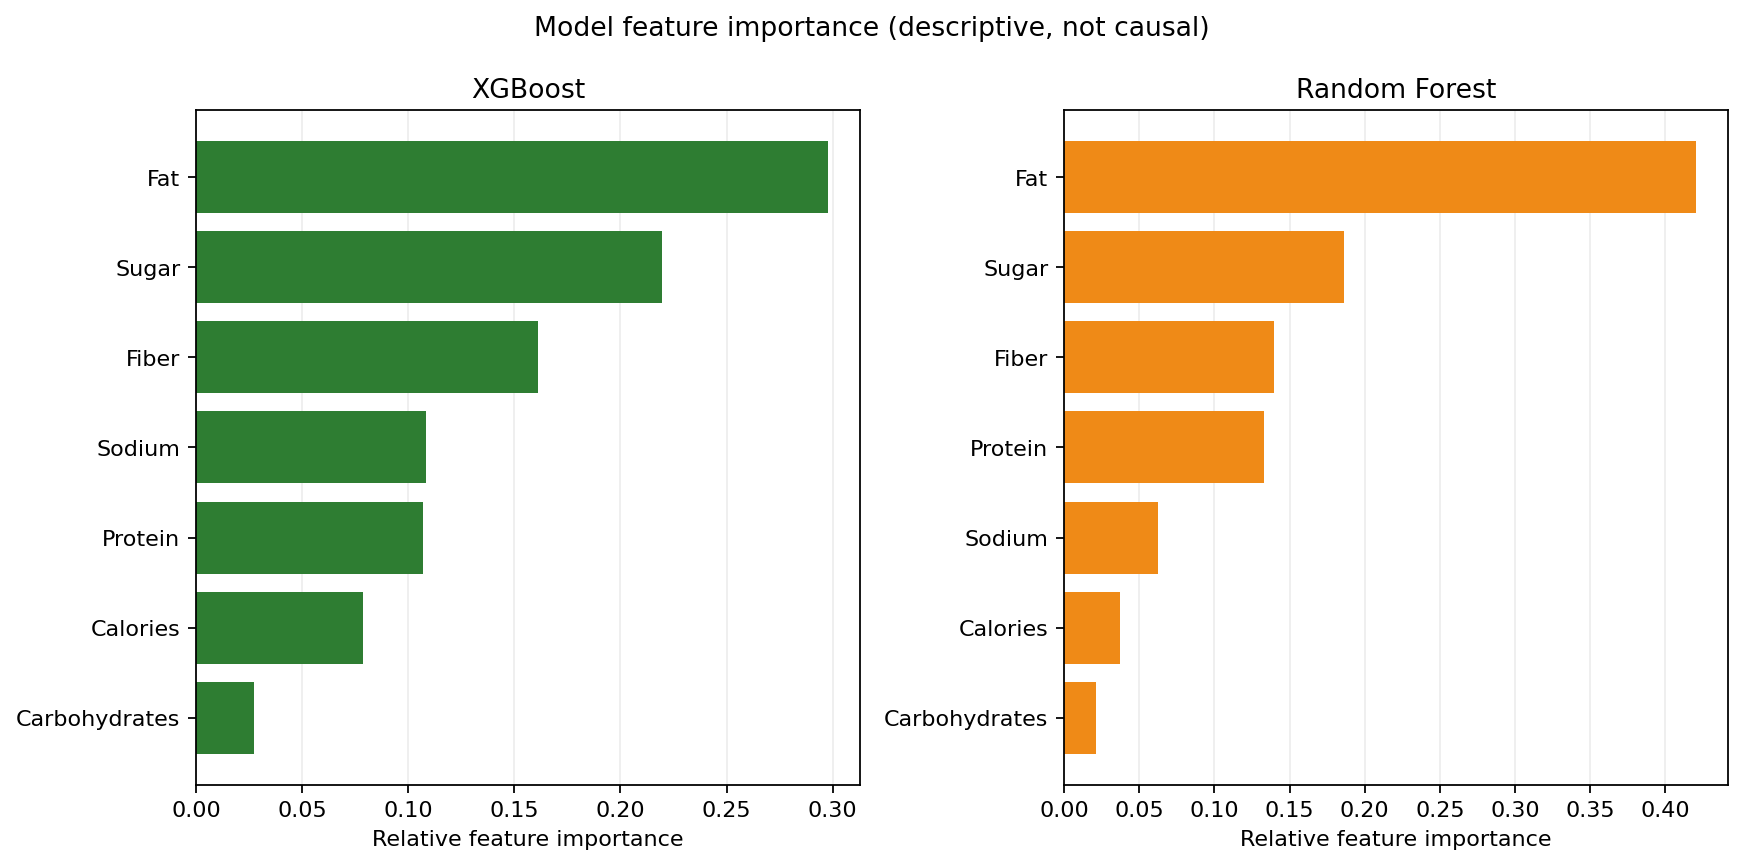
\includegraphics[width=0.82\textwidth,height=0.34\textheight,keepaspectratio]{recommendations/ml/training_plots/feature_importance.png}
\caption{Relative feature importance reported by XGBoost and Random Forest for the seven nutrient inputs.}
\label{fig:feature-importance}
\end{figure}

\section{Interpretation and Limitations of the Evaluation}
The high holdout metrics must be interpreted against the target definition. Since the
target is computed directly from the same seven nutrition fields supplied as features,
the task is to approximate a known formula. It is not evidence that the model predicts
health outcomes, user satisfaction, weight change, or dietitian judgments. The synthetic
boundary cases help cover score extremes but contribute only 17 of 1,060 samples. A
random row split may also place closely related foods in both subsets. No cross-validation,
independent external test set, ablation study, confidence interval, or prospective user
study is part of the current trainer.

For a stronger scientific evaluation, the next version should collect independently
reviewed suitability labels or user preference/outcome data, define a target before model
training, separate near-duplicate food groups between train and test, compare against
simple baselines, use repeated or grouped validation, and report calibration and error
analysis by food category. Until then, the primary defensible conclusion is that XGBoost
better approximates the project's current heuristic target on the tested split.

% -----------------------------------------------------------------------------
\chapter{Implementation and Current Results}
% -----------------------------------------------------------------------------
\section{Implemented User Workflows}
\begin{enumerate}
  \item Users register, authenticate, and create or update a profile.
  \item The dashboard displays today's logged nutrition and recent meal, water, and
        weight activity.
  \item Users select foods or variants, enter a gram portion, and the application scales
        per-100-g nutrition values to that portion.
  \item The meal planner requests current eligible recommendations and supports
        combined filters for Nepali foods, vegetarian foods, protein, and preferred foods,
        plus one meal-time category.
  \item Users can quick-log a suggested food, after which the daily budget is refreshed.
  \item Users can like or dislike a food; feedback is stored per user and contributes to
        later ranking signals.
  \item The chatbot can retrieve profile/allergy information, recent meals, current food
        suggestions, and saved likes/dislikes through server-side tools.
\end{enumerate}

\section{Principal Data Models}
The primary models are \texttt{UserProfile}, \texttt{Food}, \texttt{FoodVariant},
\texttt{MealLog}, \texttt{WaterLog}, and \texttt{WeightLog}. The recommendations app
adds \texttt{RecommendationHistory}, which associates a user and food with feedback,
score, and whether it was eaten. Food rows retain category, nutritional values, serving
information, food-type labels, eligibility flags, provenance, and recommendation group.

\section{API and Application Routes}
The web application includes registration, login, profile, dashboard, and chatbot routes.
The recommendations application provides the meal-planner page, an authenticated GET
recommendations endpoint, a feedback endpoint, and an authenticated quick-log endpoint.
The recommender returns at most 24 results after applying the eligibility and requested
filters.

\section{Conversational Assistant Use Cases}
The chatbot accepts nutrition questions through a session-backed conversation page. A
typical interaction has three parts: the user asks a question in natural language; the
Groq model determines which application data is needed and requests the corresponding
function; and the server executes that function for the current authenticated user before
the model writes its response. This design allows the same interface to answer questions
about profile constraints, past meals, food preferences, and current suggestions without
placing database access in the browser.

\begin{table}[H]
\centering
\caption{Example chatbot questions and supporting tool calls}
\begin{tabularx}{\textwidth}{p{0.40\textwidth}p{0.48\textwidth}}
\toprule
Example user question & Tool-supported context\\
\midrule
``What did I eat this week?'' & Recent meal records, dates, portions, calories, and
macros for the authenticated user.\\
``Which foods have I liked or disliked?'' & Saved liked and disliked foods from that
user's recommendation feedback history.\\
``Suggest something for lunch that avoids my allergies.'' & Profile allergies and current
recommendations from the filtered meal-planner engine.\\
``Can you suggest something similar to foods I like?'' & Preference history followed by
current recommendation results; exact historical display lists are unavailable.\\
\bottomrule
\end{tabularx}
\end{table}

Tool outputs provide context rather than forcing the model to invent database facts.
Numerical totals returned by the tools are the application's stored values. The model's
response remains generated text, so the interface and system prompt make clear that the
assistant provides general guidance rather than diagnosis or treatment. If the external
API is unavailable or unconfigured, the Django view displays an error message rather than
pretending a tool request succeeded.

\section{Functional Testing}
The explicit Django tests check the following feature groups:

\begin{table}[H]
\centering
\caption{Automated functional test coverage}
\begin{tabularx}{\textwidth}{p{0.29\textwidth}cX}
\toprule
Feature group & Tests & Representative checks\\
\midrule
CSV catalog import & 1 & Label mapping, stale-catalog eligibility, stable IDs for
duplicate names.\\
Dashboard food logging & 1 & Gram portions, scaled calories/macros, displayed daily
calories.\\
Personal nutrition targets & 2 & Goal-relative TDEE targets and weight-based macros.\\
Chatbot data and tools & 5 & Selected/custom allergies, user-scoped meal history,
allergen-safe ideas, preferences, multi-step tool calling.\\
Recommendations and quick logging & 5 & Eligibility, combined filters, API parameters,
CSRF, portion scaling, and refreshed daily budget.\\
Training plots & 1 & All four chart files are generated and non-empty.\\
\midrule
Total & 15 & Functional regression tests across the principal user workflows.\\
\bottomrule
\end{tabularx}
\end{table}

On 18 November 2026, the following command completed with all 15 tests passing and
Django reporting no system-check issues:
\begin{verbatim}
python manage.py test myapp.tests recommendations.tests
\end{verbatim}

These are functional tests. They do not substitute for external nutrition validation,
clinical review, user acceptance testing at scale, security review, load testing, or
long-term recommendation effectiveness measurement.

% -----------------------------------------------------------------------------
\chapter{Discussion, Limitations, and Future Work}
% -----------------------------------------------------------------------------
\section{Current Limitations}
\begin{enumerate}
  \item \textbf{Catalog provenance:} the CSV retains source labels, but original source
        URLs, licenses, retrieval dates, and verification records are not uniformly
        available for every row.
  \item \textbf{ML target validity:} the nutrition-quality label is a weighted heuristic
        generated from the same features used by the regressors. The model approximates
        that rule rather than learning verified human judgments.
  \item \textbf{Validation scope:} the reported metrics come from one seeded random
        split, and the dataset is a mixture of real catalog entries and a small set of
        synthetic boundary records.
  \item \textbf{Nutrition model scope:} BMR/TDEE and macro targets are estimates. BMI
        is not implemented in the current code despite appearing in the mid-term report.
        Users with incomplete profiles may receive fallback values.
  \item \textbf{Allergen coverage:} hard filtering depends on food allergen tags and
        user-entered allergies. Missing or incorrect source tags can leave unsafe records
        unidentified; this is not a guarantee of allergen safety.
  \item \textbf{Recommendation history:} the application stores feedback, not every
        recommendation impression. It cannot provide an exact archival list of all cards
        previously displayed.
  \item \textbf{Conversational grounding:} the assistant uses backend function tools but
        no vector-store RAG corpus. Its natural-language response can still be incorrect;
        tool outputs and deterministic calculations remain the source of application data.
\end{enumerate}

\section{Future Work}
\begin{enumerate}
  \item Verify source URLs, licenses, collection dates, and nutrition units for each
        catalog record and retain them with the relevant source label.
  \item Replace formula-derived ML labels with expert-reviewed suitability labels or
        carefully collected preference/outcome data; keep safety eligibility as explicit
        deterministic rules.
  \item Conduct grouped cross-validation and independent evaluation, report category-
        specific errors, compare the model with the formula baseline, and track model
        versions and dataset hashes.
  \item Add recommendation-impression logging if the product needs historical answers
        about exactly which recommendations were shown.
  \item Add integration, usability, deployment, privacy, and security testing; manage API
        credentials and production settings outside source code.
  \item Consider BMI only after defining how it will be presented and clinically
        contextualized; it should not be presented as a diagnosis.
  \item Evaluate portion conversions, recipe-specific serving definitions, and food
        database allergens with nutrition experts.
\end{enumerate}

\section{Conclusion}
NutriAI has progressed from a mid-term prototype to an integrated application with a
1,475-row labeled runtime catalog, profile-derived energy targets, gram-based logging,
rule-based food eligibility, live filtered recommendations, saved preference signals,
and a tool-enabled conversational assistant. A reproducible comparison on the current
heuristic target favors XGBoost over Random Forest on the reported fixed holdout split.
The central qualification is that this is a prototype nutrition recommender, not a
clinically validated system: the model target is formula-generated, data provenance must
be verified per record, and recommendation quality requires independent expert and user
evaluation.

% -----------------------------------------------------------------------------
\chapter*{Defense Questions and Short Answers}
\addcontentsline{toc}{chapter}{Defense Questions and Short Answers}
\begin{enumerate}
  \item \textbf{Which model is used in the live ranking?} XGBoost is the primary
        quality-score model. Random Forest is trained and scored for comparison, but the
        live hybrid formula uses the XGBoost score, budget fit, and preference signal.
  \item \textbf{Why use an 80:20 split?} It keeps most rows for fitting while reserving a
        reproducible holdout for an initial check. It is a baseline choice, not proof of
        generalization; grouped or repeated validation is future work.
  \item \textbf{What loss is minimized?} Both estimators are regressors with squared-error
        defaults. XGBoost's default objective is squared error; Random Forest's default
        split criterion is squared error. MAE, RMSE, and $R^2$ are evaluation metrics, not
        the training loss in this script.
  \item \textbf{What do the reported metrics prove?} They show how well each model
        approximates the formula-generated target on one held-out split. They do not prove
        clinical effectiveness, true food healthiness, or user satisfaction.
  \item \textbf{Why XGBoost rather than Random Forest?} On the same current split,
        XGBoost has lower regression errors and higher $R^2$, accuracy, recall, and F1;
        precision is tied. It is therefore selected as primary for this prototype.
  \item \textbf{Is this RAG?} No. The current chatbot uses server-side tool calling for
        user data and current recommendations. The repository has no vector database or
        retrieval corpus.
  \item \textbf{How was the active food dataset prepared?} Food records were extracted
        from multiple source datasets, consolidated into a fixed CSV, and cleaned to
        satisfy the project's nutrition, classification, and eligibility requirements.
        Source labels are retained in the catalog for traceability.
  \item \textbf{Is BMI implemented?} Not in the current code. It was mentioned in the
        mid-term report, but should be treated as future work unless implemented and
        tested.
\end{enumerate}

% -----------------------------------------------------------------------------
\begin{thebibliography}{99}
\bibitem{armand2024} T. P. T. A. Armand, K. A. Nfor, and J.-I. Kim,
``Applications of artificial intelligence, machine learning, and deep learning in
nutrition: A systematic review,'' \emph{Nutrients}, vol. 16, no. 7, p. 1073, 2024.
\bibitem{bondevik2024} J. N. Bondevik, K. E. Bennin, O. Babur, and C. Ersch,
``A systematic review on food recommender systems,'' \emph{Expert Systems with
Applications}, vol. 238, p. 122166, 2024.
\bibitem{sefa2021} S. M. Sefa-Yeboah et al., ``Development of a mobile application
platform for self-management of obesity using artificial intelligence techniques,''
\emph{International Journal of Telemedicine and Applications}, vol. 2021,
Art. 6624057.
\bibitem{samad2022} S. Samad et al., ``Smartphone apps for tracking food consumption
and recommendations: Evaluating artificial intelligence-based functionalities,
features and quality of current apps,'' \emph{Intelligent Systems with Applications},
vol. 15, p. 200103, 2022.
\bibitem{kim2024} D. W. Kim et al., ``Qualitative evaluation of artificial
intelligence-generated weight management diet plans,'' \emph{Frontiers in Nutrition},
vol. 11, Art. 1374834, 2024.
\bibitem{breiman2001} L. Breiman, ``Random forests,'' \emph{Machine Learning},
vol. 45, pp. 5--32, 2001.
\bibitem{chen2016} T. Chen and C. Guestrin, ``XGBoost: A scalable tree boosting
system,'' in \emph{Proceedings of the 22nd ACM SIGKDD International Conference on
Knowledge Discovery and Data Mining}, pp. 785--794, 2016.
\bibitem{mifflin1990} M. D. Mifflin et al., ``A new predictive equation for resting
energy expenditure in healthy individuals,'' \emph{The American Journal of Clinical
Nutrition}, vol. 51, no. 2, pp. 241--247, 1990.
\bibitem{nepalFCT} Department of Food Technology and Quality Control, Nepal,
\emph{Nepal Food Composition Table 2012}, 2012. The live CSV provenance field
identifies this source for 498 records; record-level verification remains necessary.
\end{thebibliography}

\end{document}
